%Section: "Diffusivities"  (Jeff, Chris C., Chris R.)
    %       -details of two approaches
    %       -notable "fudge factors" in each (timestep in Bayesian approach, integration cutoff in Langevin/Hummer method)
    %       -using US windows for Hummer method vs. separate simulations with higher restraint
    %       -can diffusivity ever really be known?  (hints at breakdown of solubility-diffusion model)

    \section*{Diffusivities}
    \par The second key component of the solubility-diffusion model is the position-dependent diffusivity, $D$($z$). However, some commonly used methods for estimating diffusivity from simulations are not applicable to the heterogeneous membrane environment. One of the most common means of calculating the diffusion coefficient of a solute dissolved in a liquid is the Einstein--Smoluchowski equation. In the one-dimensional long-time limit, this equation relates the diffusivity, $D$($z$) to the mean square deviation of the position of the solute,
    \begin{equation}
    D(z) = \frac{\langle \left| z(t) - z(0) \right|^2 \rangle}{2t}.
    \label{eq:einstein-smoluchowski}
    \end{equation}
    This relationship is only valid for solutes undergoing a random walk in a homogeneous liquid and offers a very poor approximation of the true diffusivity in a membrane, where most solutes encounter free-energy barriers with heights greater than $k_\mathrm{B} T$. For similar reasons, estimates based on a Green--Kubo relation of the velocity are expected to be equally poor\cite{Mamonov2006}. 
    
    \par Marrink and Berendsen calculated the diffusivity profile for the permeation of water using the force autocorrelation function,\cite{Marrink1994,Marrink1996}
    \begin{equation}
    D(z) = \frac{(k_\mathrm{B} T)^2}{\displaystyle \int_0^\infty \langle {\Delta}F_z(z,t)  {\Delta}F_z(z,0) \rangle \textrm{d}t}.
    \label{eq:diff_marrink}
    \end{equation}
    This method requires that the solute be constrained to a point $z$ on the coordinate, which makes it relatively difficult to apply because the equations of motion of the MD integration must be modified to impose the constraint.\cite{Wilson1985,Mamonov2006} As a result, it is far more common to perform simulations where the solute is simply restrained to remain near a given value of $z$ with a biasing potential. As the solubility-diffusion model requires the determination of $W$($z$) and $D$($z$) over the full bilayer, it would be preferable for the method used to provide both of these profiles from one set of simulations.

    \par In the following sections, we present two strategies for calculating $D$($z$) for the permeation of a solute across a lipid bilayer using biased MD simulations. The first is based on the generalized Langevin equation for a harmonic oscillator. The second employs Bayesian inferences on the likelihood of the observed dynamics of the solute.

    \subsection*{The Generalized Langevin method}
    %%\subsection*{Theory: Generalized Langevin equation for a harmonic oscillator approach}
    \par The generalized Langevin equation provides straightforward methods to calculate 
    position-dependent diffusion coefficients from restrained MD simulations. In these methods, the solute is restrained by a harmonic potential so that it oscillates at a point along the coordinate. The solute can now be described as a harmonic oscillator undergoing Langevin dynamics, where the remainder of the system
    %{\bf the balance of the system} 
    % YW: mmm... what is the balance of the system?
    % JC: my guess: "balance" means "everything else"
    serves as the frictional bath for the solute. Implicitly, describing the system as a harmonic oscillator requires the restraining potential to be dominant over the underlying free energy surface, i.e., the latter is effectively a perturbation on the former.
    %If the underlying free-energy surface is rough, 
    Otherwise, 
    the assumption that the bilayer serves only as a frictional bath to the oscillating solute may not be valid.  Values of the spring constant sufficiently large to justify this assumption also tend to be too large for umbrella sampling simulations, meaning that it may not be possible to use the same simulation to calculate $W$($z$) and $D$($z$).

    \par Once a time series of the $z$ position of the solute is collected, the diffusion coefficient for that point can be calculated from the position or velocity autocorrelation functions (ACF and VACF, respectively).  These methods were originated by Berne and coworkers for the calculation of reaction rates\cite{Berne1988}, and elaborated by Woolf and Roux to calculate position dependent diffusion coefficients.\cite{Woolf1994} In their approach, the diffusion coefficient is calculated from the VACF. This approach requires the numerical Laplace transform of the VACF for several values of the transform parameter $s$ and extrapolation to the limit of $s=0$. Hummer proposed a simpler method to calculate diffusion coefficients from harmonically restrained simulations\cite{Hummer2005} in which the diffusion coefficient is calculated directly  from the integral of the ACF, $C_{zz}$, of $z$ and the variance of $z$,

    \begin{equation}
    D(z= \langle z \rangle ) = \frac{\textrm{var}(z)^2}{\displaystyle \int_0^\infty C_{zz}(t) \, \textrm{d}t}.
    \label{eq:diff_hummer}
    \end{equation}

    \par This method is attractive because it is simple to impose a harmonic restraint on a solute and save a time series of the $z$-position of this trajectory in most MD codes. It also avoids the need for multiple numerical Laplace transforms of the VACF. The ACF can be calculated directly from this time series,\cite{Allen1989}
    \begin{equation}
    C_{zz}(t) =  \langle \delta z(0) \delta z(t) \rangle = \frac{1}{n_\mathrm{samples}}\sum\limits_{i=0}^{n_\mathrm{samples}} \delta z(i) \delta z(t+i)
    \label{eq:correlation_sum}
    \end{equation}
    where $\delta z(t) = z(t)-\langle z \rangle$. Our code for calculating the ACF from a NAMD\cite{Phillips2005}
    %Colvars\cite{Fiorin2013} 
    time series is provided in the SI. 
    %available for download (Ref. \citenum{ACFCalculator}). 
    Although this method is a straightforward way to calculate membrane diffusion coefficient profiles, there are several practical issues associated with its use. We illustrate these issues by presenting the ACFs calculated from a simulation of urea restrained at three positions in the model bilayer system: $z=0$ \AA, $z=10$ \AA, and $z=36$ \AA\ (see Fig.~\ref{fig:acf}).

    \begin{figure}
    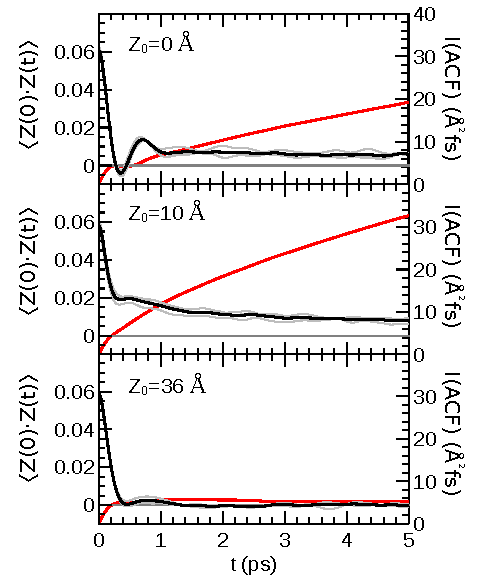
\includegraphics[width=0.65\textwidth]{Figures/acf-stacked}
    \caption{Time autocorrelation function of urea in the model DMPC bilayer 
    restrained at various values of $z_0$ using a harmonic potential 
    ($U_\mathrm{rest}=\frac{1}{2}k(z-z_0)^2$, $k=10$ kcal/(mol \AA$^2$)). 
    The black lines are the cumulative ACF calculated from three 1-ns simulations. 
    The ACF from each 1-ns trajectory alone is presented in grey. The red lines 
    (secondary axis) show the integral of the ACF over the interval $[0,t]$.}
    \label{fig:acf}
    \end{figure}

    \par Correlation functions typically require extensive sampling to achieve convergence, particularly for long correlation times. Heterogeneity of the bilayer environment can cause the ACF calculated from different simulations at the same $z$-reference value to be significantly discrepant, a particularly serious for hydrogen-bonding solutes that remain partially coordinated by water molecules inside the membrane such as urea (see Fig. S3). This issue can be addressed in part by performing several simulations, with a long equilibration period for each. The correlation functions can then be calculated from long time series, e.g., > 1 ns, collected from each of these simulations.

  \par The general features of the ACFs can be interpreted based on the analytical solution to the autocorrelation function of a harmonic oscillator undergoing Langevin dynamics,\cite{Tuckerman2010}
\begin{equation}
C_{zz}(t) = \textrm{var}(z) e^{-\gamma(\bar \omega)t/2\mu}[ \textrm{cos}(\Omega t) + \frac{\gamma(\bar \omega)}{2 \mu \Omega } \textrm{sin}(\Omega t)]
\label{eq:analytical-acf}
\end{equation}
   where $\gamma$ is the friction coefficient, $\bar \omega$ is the renormalized frequency of the oscillator, and $\mu$ is its reduced mass. $\gamma$ determines the rate of decay of the ACF. The expected behavior of the ACF based on Eq.~\ref{eq:analytical-acf} is that for damped periodic oscillations; however, if the friction coefficient, $\gamma$, is high, the ACF may decay to zero before there are any significant oscillations. This decay is apparent in the ACF when the solute is restrained at  $z=36$ \AA\ (bulk water; see Fig.~\ref{fig:acf}), which decays to zero within 0.5 ps, but then has a short second peak extending to 1.2 ps. The calculation of the diffusion coefficient formally requires the integration of the ACF in Eq.~\ref{eq:diff_hummer} over the interval $[0, \infty]$, but the ACF will  decay to zero within $\sim$ 2 ps in most fluid environments. Even if extensive sampling has been performed, there can be significant noise in the ACF at long times. Hummer noted that this noise causes the calculated diffusion coefficients to be sensitive to the interval of integration.\cite{Hummer2005} The g\_wham code~\cite{Hub2010}, one of the tools provided with Gromacs, limits the contribution of noise by cutting off the integration when the ACF drops below a threshold value of $0.05\ \times\ \textrm{var}(z)$.  This cutoff is not appropriate in all instances because the ACF can go through multiple oscillations before converging to zero. Nevertheless, it can provide reasonably accurate results if the autocorrelation function decays rapidly (i.e., in a high friction regime).

  \par Compared to bulk water, the autocorrelation functions in the lipid tail region are much slower to converge.  The ACFs from simulations with $z_0=10$ \AA\ and $z_0=0$ \AA\ only decay to 8 and 13\% of their initial values in 5 ps, respectively. A consequence of the 
failure to converge to zero is that the integrated ACF increases almost linearly, 
% what pateau?
%once the plateau is reached. This 
causing the calculated diffusion coefficients to be sensitive 
to the interval over which the ACF is integrated.  Typically, this sensitivity will cause 
the integrated ACF to be larger than it should be, so that the calculated diffusion coefficient is erroneously underestimated.

The slow convergence of the ACF is consistent with the work of Neale et al.,\cite{Neale2011} 
which showed that the convergence of US simulations of solute permeation 
into bilayers can require $\mu$s-ms-length simulations. Long correlation times are 
due to slow diffusion of the lipid tails, variations in the hydration of the solute, and
inhomogeneities in the bilayer interface that form over very long time scales.\cite{Neale2013}
While US simulations of the bilayer PMF can achieve convergence by running for a very long time, the 
lack of ergodicity in sampling is inconsistent with the underlying model of harmonic 
oscillator in frictional bath that is used to derive Eq.~\ref{eq:diff_hummer}.

The issues noted above for calculating diffusivity in the membrane are typically not 
significant for small solutes like water,\cite{Riahi2014,Issack2015} 
but they are severe for larger, more complex ones, such as urea, which are more prone to 
have long-time correlations. Under such circumstances, the Generalized Langevin method is not appropriate for 
calculating $D$($z$).  To determine if convergence issues are significant for a given 
system, the ACF should be calculated and plotted for several $z$-positions in the bilayer. If the ACF 
has not decayed to values near zero at long time scales (e.g., 5 ps), the Generalized Langevin 
method is probably not appropriate for calculating the position-dependent diffusivity for that solute. 

In the Generalized Langevin approach, a prerequisite noted above is that the force constant 
of the harmonic restraint should be sufficiently large to render the underlying free-energy 
surface a small perturbation on the harmonic potential.  The force constant used for the US 
simulations, 1.5\,kcal/mol/\AA$^2$, may be 
too small for application of this approach.  To test its applicability, we ran additional 
2-ns simulations for each window for urea using a much larger restraining force constant 
of 10\,kcal/mol/\AA$^2$.  However, as shown in Fig.~S6, the differences 
between the $D$($z$) profiles for the two cases are practically negligible at nearly all 
points.  At a few data points in the membrane interior, urea under a higher restraint 
gives a diffusivity as much as twice that of urea under a lower one.  Yet, because 
the permeability depends linearly on $D$($z$) (see Eq.~\ref{eq:solubility-diffusion}), but 
exponentially on $W$($z$), even a factor of two in the diffusivity across the entire permeation 
pathway contributes only $\sim$0.3 to log\perm.  Thus, for permeability calculations, it is 
acceptable to use the same simulations for calculation of both $W$($z$) and $D$($z$).

\subsection*{The Bayesian inference method}

%the accuracy of the approximation depends both on the strength
%of the confining potential and the magnitude of undulations
%in the intrinsic potential of mean force.

A fundamentally different approach for the determination of position-dependent 
diffusivities employs Bayesian inferences to reconcile thermodynamics and kinetics\cite{Hummer2005,Turkcan2012,Comer2013}.  This approach is especially suited for calculations within lipid membranes
because no assumptions are made regarding the form of the free-energy landscape on which diffusion occurs.
Furthermore, such an approach
is compatible with a wide variety of biasing schemes used in MD,
and thus, allows the practitioner more flexibility in simulation design.
This approach may be viewed as the
inverse solution of the Smoluchowski equation, which yields consistent estimates
of $W$($z$) and $D$($z$), given the
trajectory obtained from biased simulations.
These biases may also be time-dependent, as is the case for
the metadynamics and ABF algorithms.
Since the latter free-energy calculation algorithms are
designed for the accurate description of $W$($z$), one may use it as a
consistency check of the solution provided by the Bayesian inference method.
Alternatively, $W$($z$) as determined by a free-energy algorithm can
serve as a prior in the Bayesian scheme, increasing the reliability of
$D$($z$) in situations where statistics are poor.
In a nutshell, the Bayesian scheme uses as parameters the values of
the transition coordinate, $z$, along the trajectory, together with the force, $F(z,t)$,
which is the sum of the time-dependent bias and the intrinsic system force, equal
to $-\nabla W(z)$. Under the stringent assumption of a diffusive regime, the 
motion is propagated using a discretized Brownian integrator,
%
%% \begin{equation}
%% \label{Brownian}
%% \Delta z = z_2(t) - z_1(t) = \beta D(z_1) F(z_1, t_1) \Delta t + \nabla D(z_1) \Delta t + \sqrt{2 D(z_1) \Delta t} \ g(t) 
%% \end{equation}
\begin{equation}
 \Delta z = z_2(t) - z_1(t) = \beta D(z_1) F(z_1, t_1) \Delta t + \nabla D(z_1) \Delta t + \sqrt{2 D(z_1) \Delta t} \ g(t)
\label{Brownian}
\end{equation}
%
where $\beta = (k_B T)^{-1}$, $\Delta t = t_2 - t_1$ and $g(t)$
%is a Wiener process
%% (A Wiener process is an integral over Gaussian white noise, so the cumulative sum of many g(t))
is a Gaussian white noise of zero mean and variance equal to unity. Propagation along the
transition coordinate can be recast as the sum of a drift and a noise
term, i.e., $\Delta z = \mu + \sigma g(t)$, where
$\mu$ and $\sigma^2$, the variance, are defined by,
%
\begin{equation}
\left\{
\begin{array}{lcl}
\mu      & = & \beta D(z_1) F(z_1, t_1) \Delta t + \nabla D(z_1) \Delta t
\\
\sigma^2 & = & 2 D(z_1) \Delta t
\end{array}
\right.
\end{equation}
%
Propagation of motion obeys a Gaussian-distributed probability of observing the 
transition from $z_1$ at time $t_1$ to $z_2$ at time $t_2$,
%
\begin{equation}
\label{eq:Gaussian}
P[(z_2, t_2 | z_1, t_1) | F(z,t), D(z)] =
\frac{1}{\sigma \sqrt{ 2 \pi}}
\exp \left(-\frac{(\Delta z - \mu)^2}{2 \sigma^2} \right) 
\end{equation}
%
which assumes the system is in the overdamped Langevin dynamics regime and satisfies the 
fluctuation-dissipation theorem.
It is worth noting that in contrast with related
schemes, the present formalism, embodied in Eq.~\ref{Brownian}, features 
a gradient term, $\nabla D(z_1) \Delta t$, which has been shown to improve 
the accuracy of the predicted intrinsic system force, or gradient of the PMF.
%
See the SI for more details on applying the scheme 
to MD simulations.

As shown in Fig.~\ref{fig:acf}, the motion of permeants within the membrane is complex and correlations in such motion are much longer in the membrane environment than in solutions (at least several picoseconds).
These long correlation times complicate calculating the diffusivity by most
available methods, including the Bayesian inference method described herein.
A crucial component of this scheme is the time step, $\Delta t$.
%, which ought to be chosen with utmost care.
The correlations shown in Fig.~\ref{fig:acf} violate the assumptions of
overdamped Brownian motion leading to Eq.~\ref{Brownian}; thus, 
we found that $\Delta t$ values of a few picoseconds yield substantial overestimates of the diffusivity.
$\Delta t$ should be chosen to be much larger than any correlation
time of the motion; however, there is also an upper bound on $\Delta t$ because
the discretization implicit in Eq.~\ref{Brownian} requires
only small changes in $F(z_1, t_1)$ and $D$($z$) over the duration of $\Delta t$.
Errors due to the violation of this requirement are apparent when
$W$($z$) as predicted by the Bayesian scheme diverges substantially
from that obtained by the free-energy calculation technique
(here, ABF).
%We are currently developing an improved scheme to 
%remove the restrictions imposed by discretization. 
For the permeants examined in the present work,
we found $\Delta t=32$~ps still gives consistent $W$($z$)
functions while minimizing errors due to correlation.

\subsection*{Comparison of the two approaches}
As is clear from Eq.~\ref{eq:solubility-diffusion}, log\perm~is much more sensitive to $W(z)$ than to $D$($z$).
However, as shown in Fig.~\ref{fig:Dz}, there are some notable differences
in the results of the Generalized Langevin and Bayesian inference approaches, which
have an appreciable effect on the predicted permeability.
For the four methods used to determine the PMF, the Generalized Langevin approach 
for calculating $D$($z$) was used for US and REUS, while the Bayesian inference method 
was used for ABF and MW-ABF.
Under the conditions described above, i.e. the restraint strength used in the US and REUS
simulations and the $\Delta t$ chosen for the Bayesian scheme,
we obtain smaller diffusivity values using
the Generalized Langevin approach than using the Bayesian approach.
These differences are most notable near $z=0$, where the value of $D$($z$)
most influences the permeability for urea due to the maximum of $W$($z$).
For example, the much larger diffusivity of urea
near the center of the membrane as determined by the Bayesian scheme
compared to the Generalized Langevin scheme (see Fig.~\ref{fig:Dz}) 
results in the ABF and MW-ABF methods having larger log\perm~values by more than
an order of magnitude, despite the fact that the
height of the free energy barrier calculated by ABF is significantly
larger than that for the other methods (see Fig.~\ref{fig:PMFs}).
{\color{red} The generally larger $D(z)$ values given by 
the Bayesian scheme are likely due to the fact that
the scheme used in the present work is limited to relatively small values of $\Delta t$, a consequence of the Gaussian approximation for the probability profile (Eq.~\ref{eq:Gaussian}). We have found that the motion of the permeants is not strictly diffusive at the $\Delta t$ values used here and that the diffusivity appears to decrease continuously with $\Delta t$. We are currently working to improve the Bayesian scheme to overcome the limitations on $\Delta t$, which will be addressed in subsequent work.}
Hence, although it plays a less dramatic role in Eq.~\ref{eq:solubility-diffusion} than $W$($z$),
$D$($z$) is also highly influential and the approach to calculating it must be
carefully considered.


%Despite the vast differences between the two methods, 
%they produce similar results, shown in Fig.~\ref{fig:Dz} for all three permeants.  


\begin{figure}[htbp]
\begin{center}
	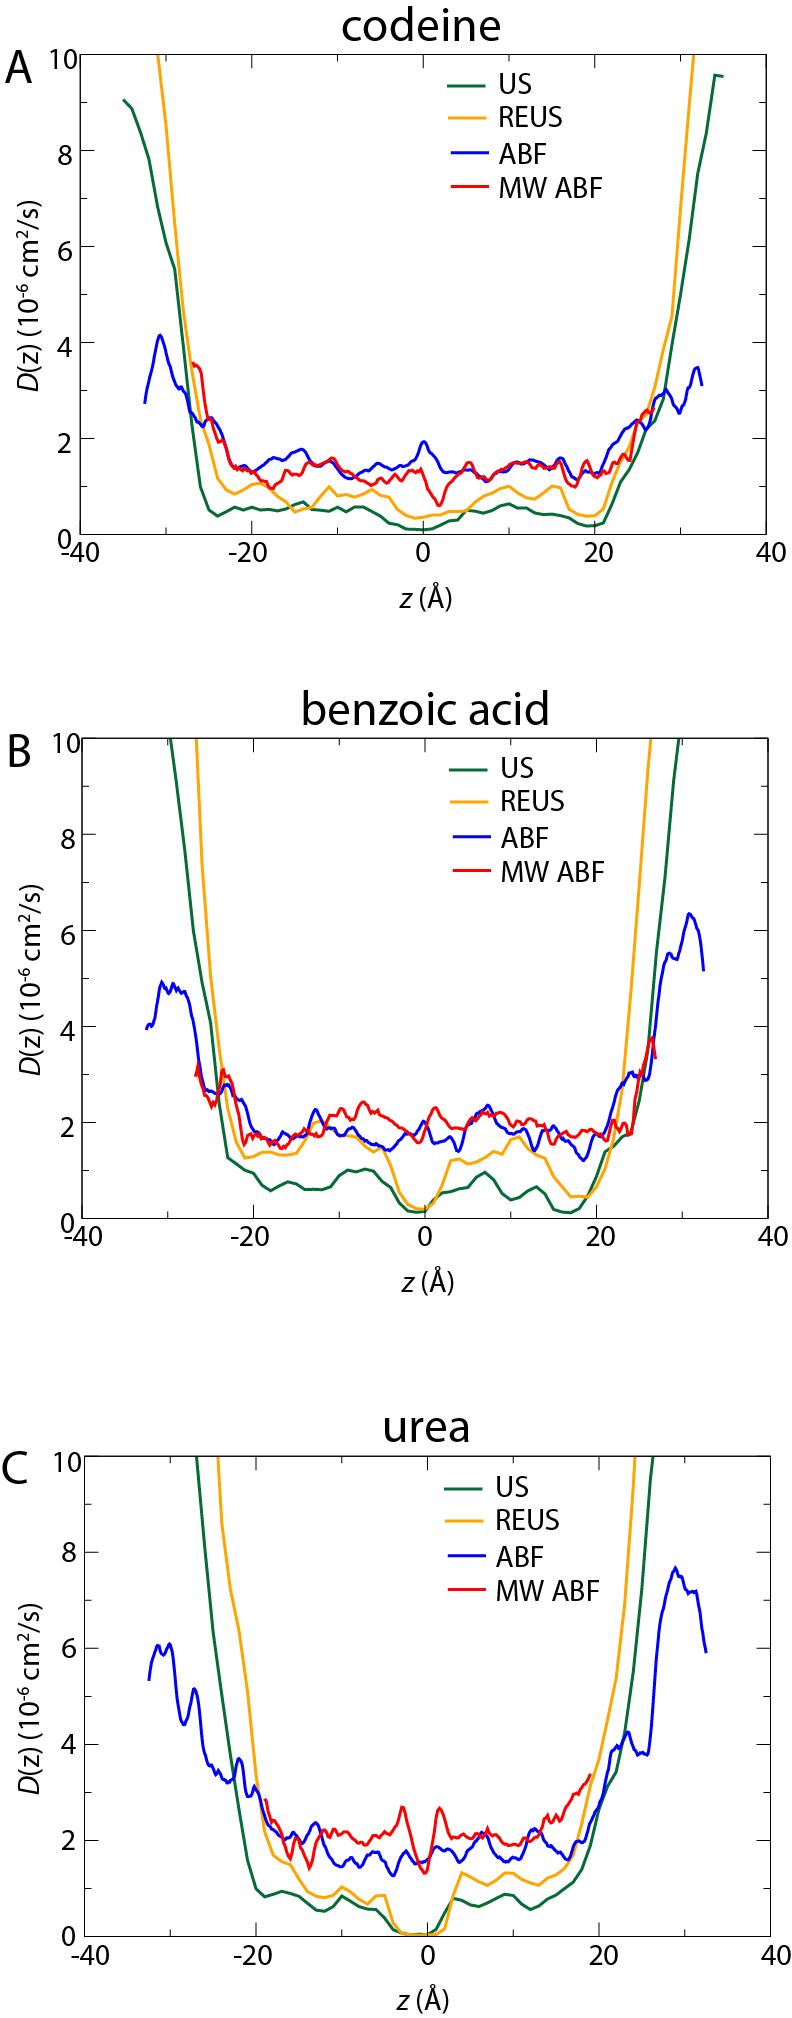
\includegraphics[width=0.4\textwidth]{Figures/Dz-all}
	\caption{Diffusivity profiles for each permeant, (A) codeine, (B) benzoic acid, and (C) urea.  In green and orange are the umbrella-based methods, US and REUS, for which the Generalized Langevin approach was used to determine $D$($z$).  In blue and red are the ABF-based methods, for which the Bayesian scheme was used.}
	\label{fig:Dz}
\end{center}
\end{figure}




% moved from end of last section


